\section{Appendix}

\subsection{Graphs for GCC-PHAT testing}\label{app:GCC-Phat-testing}
\begin{figure}[H]
    \centering
    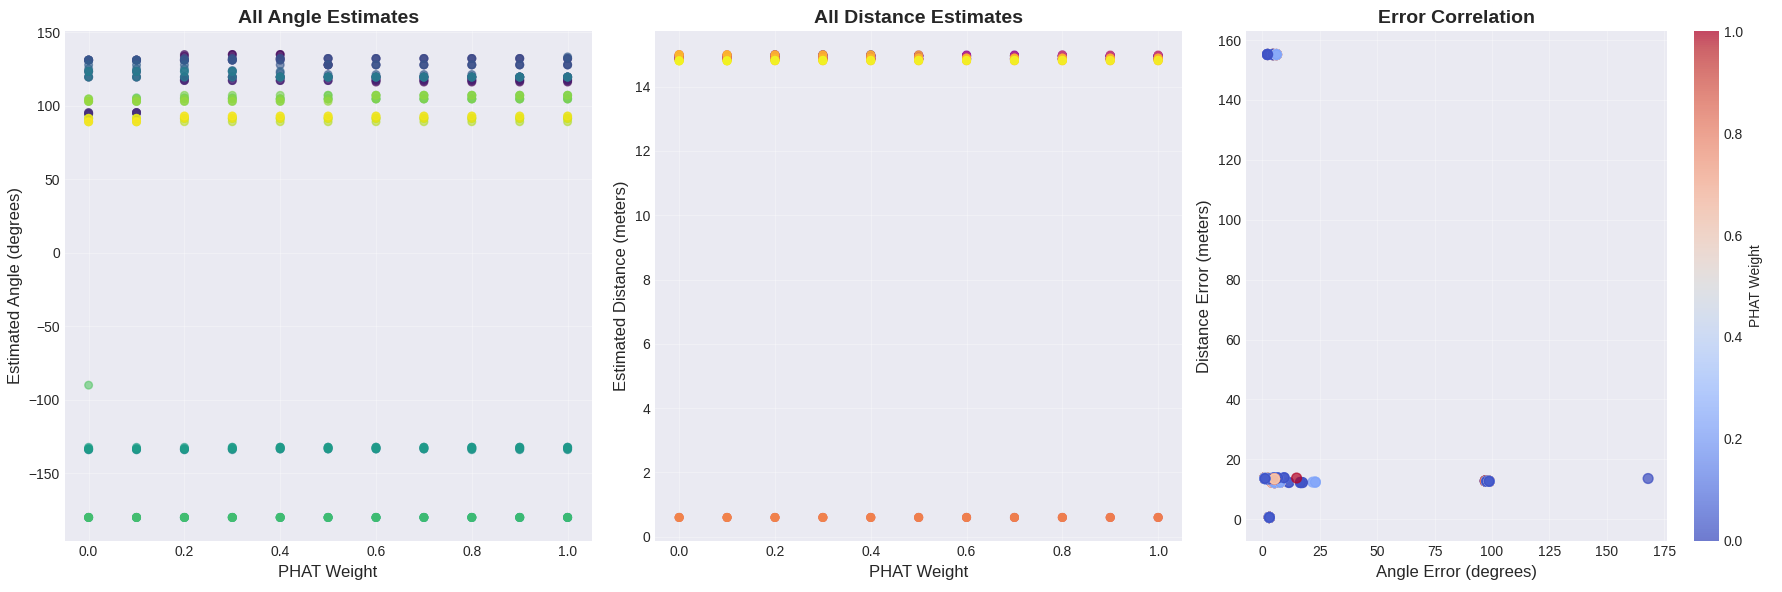
\includegraphics[width=0.8\textwidth]{Pictures/GCC-PHAT-Dot-Plot.png}
    \caption{Plots of GCC-PHAT output for different angles and distances}
    \label{fig:GCC-PHAT-Dot-Plot}
\end{figure}

\begin{figure}[H]
    \centering
    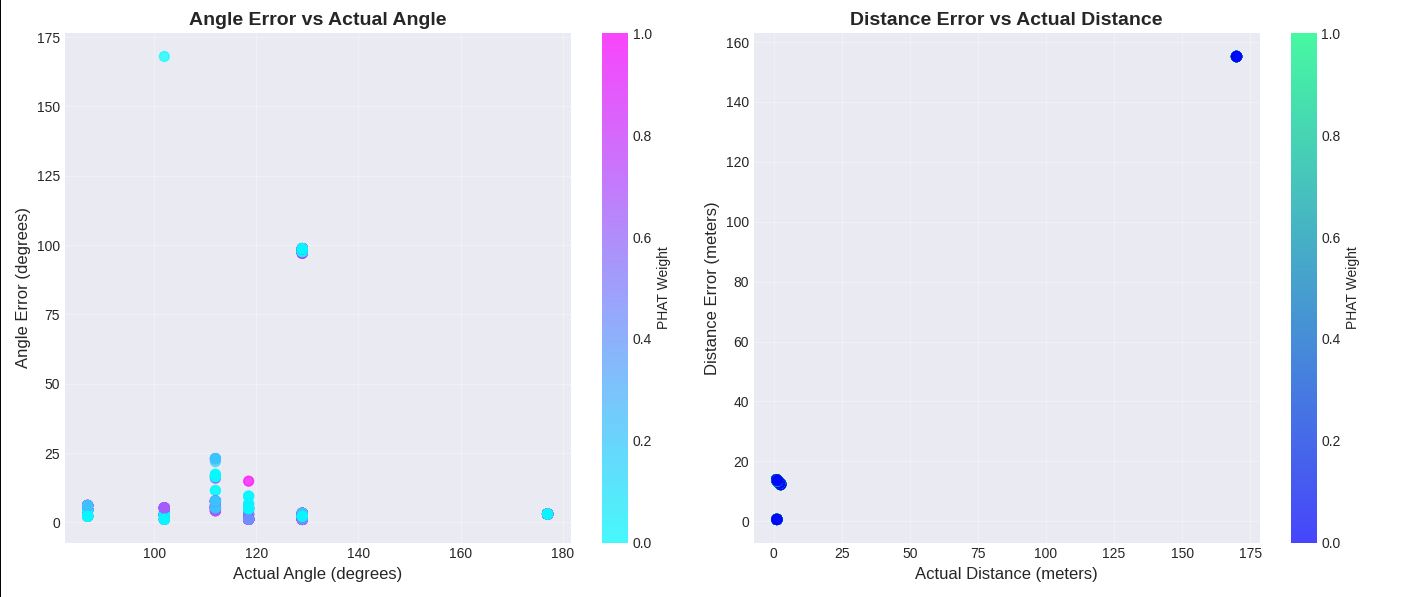
\includegraphics[width=0.8\textwidth]{Pictures/Angle-Distance-Dot-Plot.png}
    \caption{Plots of GCC-PHAT output error compared to angles and distances}
    \label{fig:Angle-Distance-Dot-Plot}
\end{figure}

\begin{figure}[H]
    \centering
    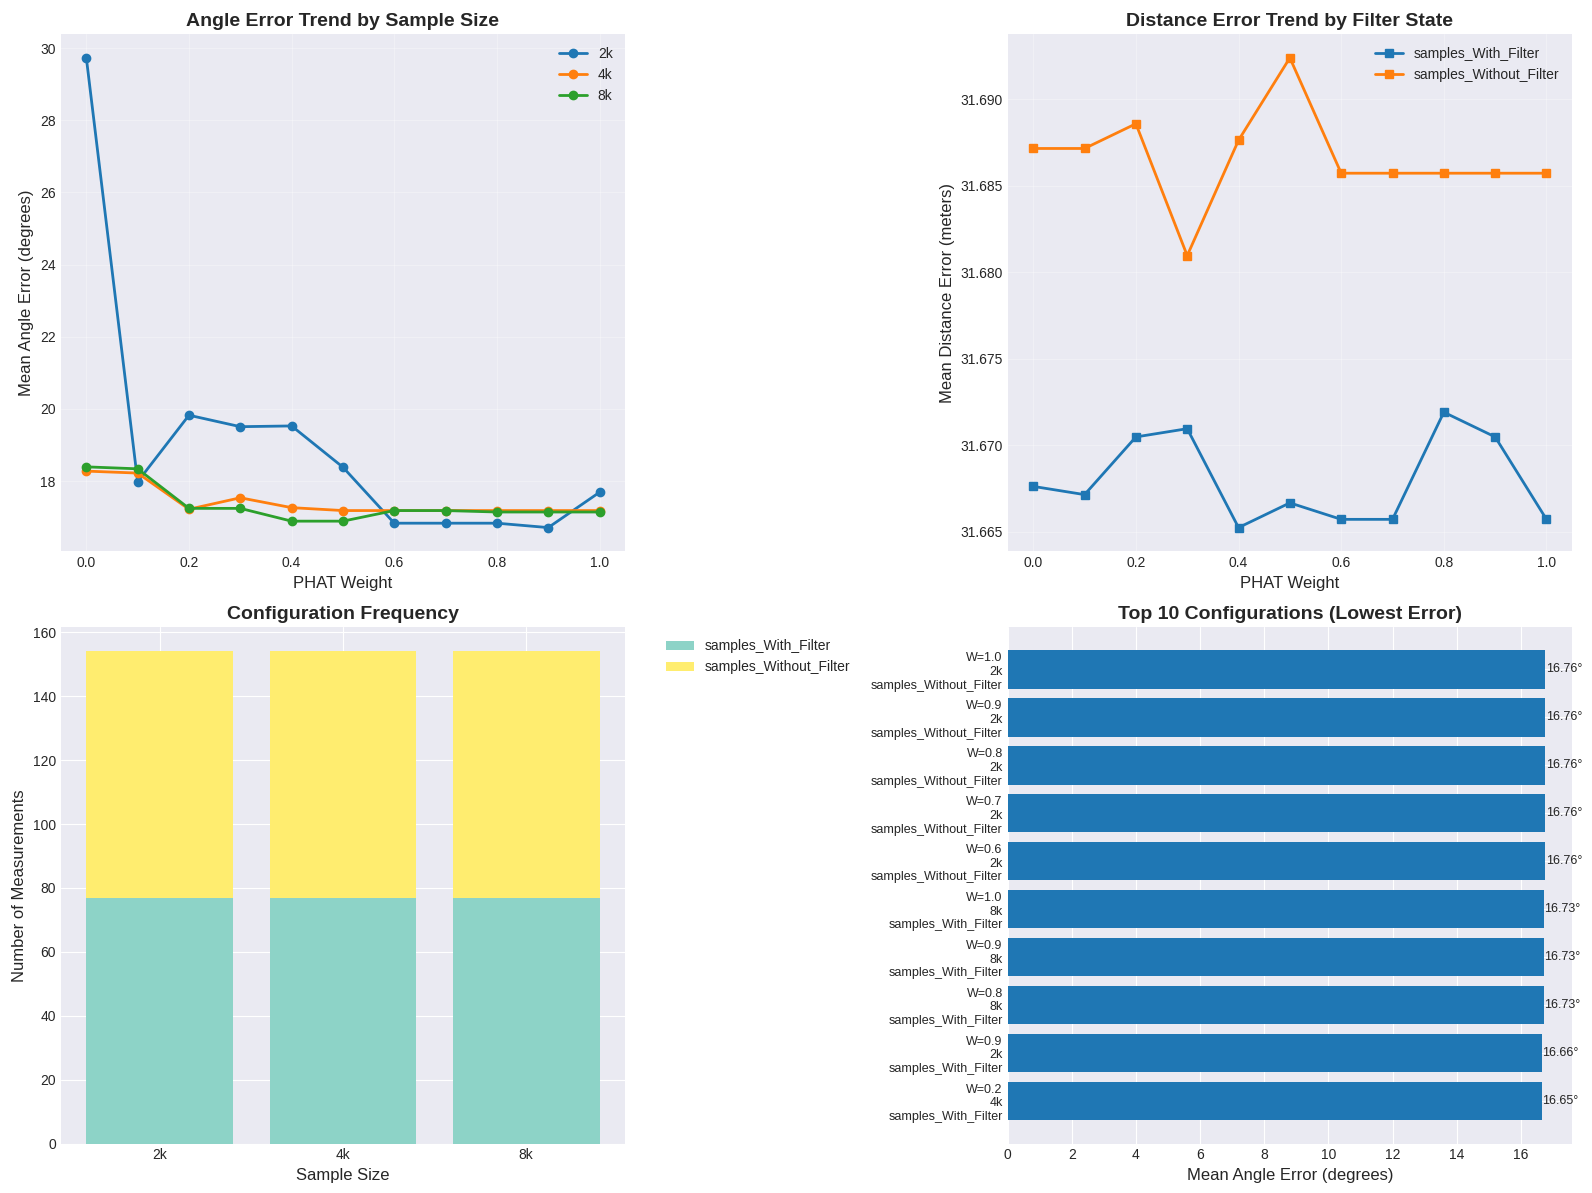
\includegraphics[width=0.8\textwidth]{Pictures/GCC-PHAT-angle-trend-and-configuration.png}
    \caption{Trends of angle error for different GCC-PHAT configurations}
    \label{fig:GCC-PHAT-angle-trend-and-configuration}
\end{figure}

\begin{figure}[H]
    \centering
    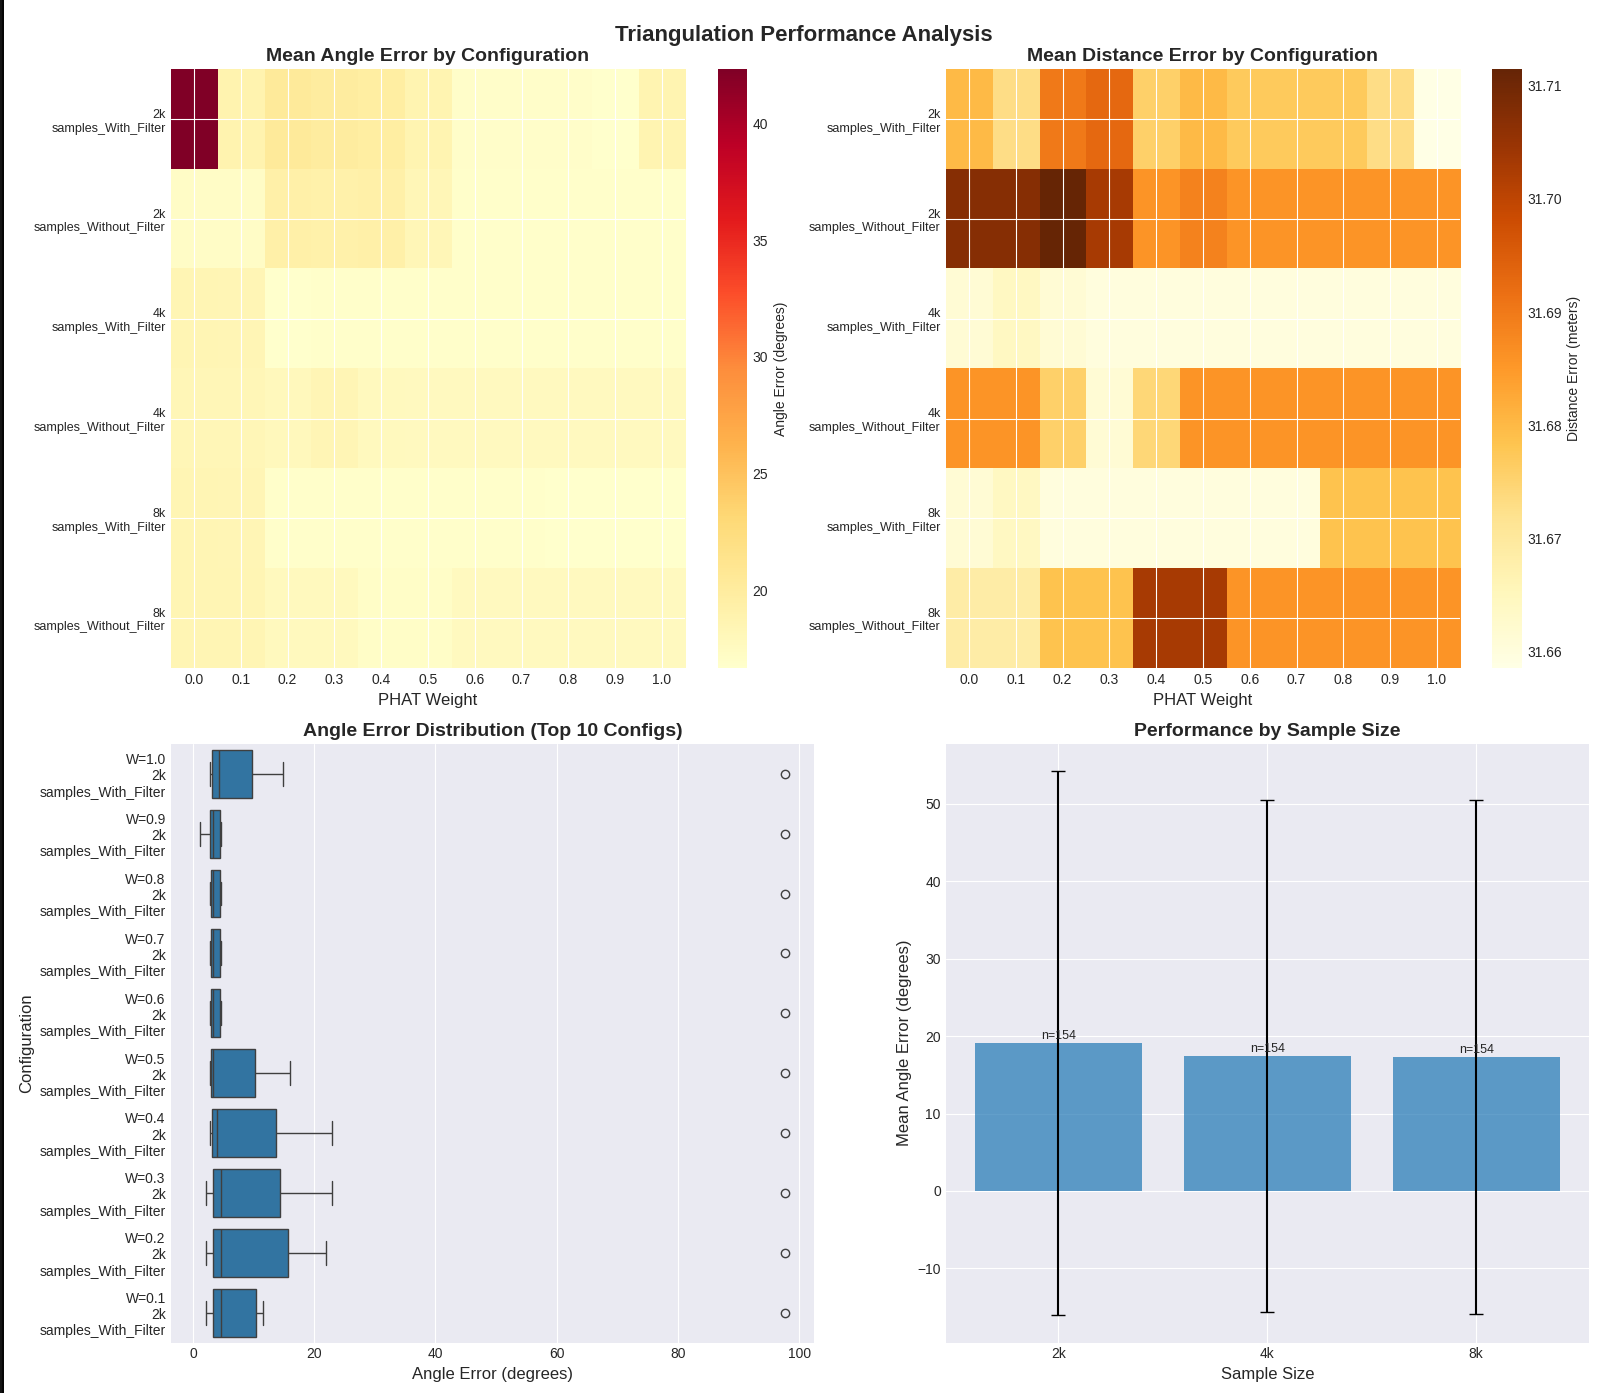
\includegraphics[width=0.8\textwidth]{Pictures/GCC-Phat-heatmaps-and-angle-distribution.png}
    \caption{Heatmaps of angle error distribution for different GCC-PHAT configurations}
    \label{fig:GCC-PHAT-heatmaps-and-angle-distribution}
\end{figure}